%% 
%% ACS project dissertation template. 
%% 
%% Currently designed for printing two-sided, but if you prefer to 
%% print single-sided just remove ",twoside,openright" from the 
%% \documentclass[] line below. 
%%
%%
%%   SMH, May 2010. 


\documentclass[a4paper,12pt]{report}


%%
%% EDIT THE BELOW TO CUSTOMIZE
%%

\def\authorname{Jonas\ Tjomsland\xspace}
\def\authorcollege{Corpus Christi College\xspace}
\def\authoremail{jt732@cl.cam.ac.uk}
\def\dissertationtitle{Continually learning social appropriateness of robot actions under uncertainty}
\def\wordcount{14,235}


%\usepackage[dvips]{epsfig,graphics} 
\usepackage{epsfig,graphicx,verbatim,parskip,tabularx,setspace,xspace}
\usepackage{mathtools}
\usepackage{amsmath}
\usepackage{amssymb}
\DeclareMathOperator{\argmin}{arg\,min}
\newcommand{\Lagr}{\mathcal{L}}

\usepackage{nomencl}
\makenomenclature

\usepackage{algorithm}% http://ctan.org/pkg/algorithms
\usepackage{algpseudocode}% http://ctan.org/pkg/algorithmicx

\usepackage{bm}

%% This code creates the groups
% -----------------------------------------
%\usepackage{etoolbox}
%\renewcommand\nomgroup[1]{%
  %\item[\bfseries
  %\ifstrequal{#1}{P}{Physics Constants}{%
  %\ifstrequal{#1}{N}{Number Sets}{%
  %\ifstrequal{#1}{O}{Other Symbols}{}}}%
%]}
% -----------------------------------------
%% START OF DOCUMENT
\begin{document}


%% FRONTMATTER (TITLE PAGE, DECLARATION, ABSTRACT, ETC) 
\pagestyle{empty}
\singlespacing
% title page information
\begin{titlepage} 

\begin{center}
\noindent
\huge
\dissertationtitle \\
\vspace*{\stretch{1}}
\end{center}

\begin{center}
\noindent
\huge
\authorname \\
\Large
\authorcollege      \\[24pt]
%\begin{figure}

\includegraphics{CUni3.pdf}
%\end{figure}
\end{center}

\vspace{24pt} 

\begin{center}
\noindent
\large
{\it A dissertation submitted to the University of Cambridge \\ 
in partial fulfilment of the requirements for the degree of \\ 
Master of Philosophy in Advanced Computer Science} 
\vspace*{\stretch{1}}
\end{center}

\begin{center}
\noindent
University of Cambridge \\
Computer Laboratory     \\
William Gates Building  \\
15 JJ Thomson Avenue    \\
Cambridge CB3 0FD       \\
{\sc United Kingdom}    \\
\end{center}

\begin{center}
\noindent
Email: \authoremail \\
\end{center}

\begin{center}
\noindent
\today
\end{center}

\end{titlepage} 

\newpage
\vspace*{\fill}

\onehalfspacing
\newpage
{\Huge \bf Declaration}

\vspace{24pt} 

I \authorname of \authorcollege, being a candidate for the M.Phil in
Advanced Computer Science, hereby declare that this report and the
work described in it are my own work, unaided except as may be
specified below, and that the report does not contain material that
has already been used to any substantial extent for a comparable
purpose.

\vspace{24pt}
Total word count: \wordcount

\vspace{60pt}
\textbf{Signed}: 

\vspace{12pt}
\textbf{Date}:


\vfill

This dissertation is copyright \copyright 2020 \authorname. 
\\
All trademarks used in this dissertation are hereby acknowledged.



\newpage
\vspace*{\fill}

\singlespacing
\newpage
{\Huge \bf Abstract}
\vspace{24pt} 

\newpage
\vspace*{\fill}


\pagenumbering{roman}
\setcounter{page}{0}
\pagestyle{plain}
\tableofcontents

\mbox{}

\printnomenclature

\listoffigures
\listoftables

\onehalfspacing

%% START OF MAIN TEXT 

\chapter{Introduction}
\pagenumbering{arabic} 
\setcounter{page}{1} 
\section{Motivation}
From a young age humans are taught appropriate behaviour through experience and observations. A misbehaving child gets feedback, helping it to gradually create an understanding of what is appropriate to do based on contextual information. Learning to navigate in a jungle of social etiquette and norms is not straightforward, a number of verbal and visual cues must be decoded and acted upon to be successful.  Not only does this takes years to learn, but even at grown age it can be difficult to accurately read and recognise the signals that indicates a social context. 

The first introduction of domestic robots was as early as 1985 \cite{breazeal2016social} but a lot has happened since then and both lawn mowing and vacuum cleaning robots are today more common household items. This progress has led to interesting developments in obstacle avoidance, localization and mapping, but the social intelligence of these robots are still far from what we would define as human-level.


In this projects we approach the challenge of taking robots one step closer to a  human-level understanding of the appropriateness of actions in such social situations. 

As humans we continuously develop this understanding

Robots are far from achieving a human-level of performance when it comes to understanding the appropriateness of actions in such social situations. The field of social robotics is well-researched, but the gap between human's and robot's social intelligence is still massive. In this work we aim to take robots one step closer to a human-like understanding of social appropriateness, by leveraging the contribution from a varied group of people and their perception of some social situations.

by giving them the ability to continuously learn and reflect upon their own knowledge. To achieve this goal we take use of state of the art probabilistic machine learning models, combined with recent advances in continual learning.

Understanding social context is non-trivial even for humans. All the small cues and indicators that must be interpreted, identifying the factors and cultural differences that might impact the social appropriateness of different actions.

Humans learn this from a young age, we continuously develop our knowledge throughout life when facing new situations and observations. We know that something that is established as socially appropriate in some cultures, might not be so in other. Often leading to us being more careful when meeting new people in new situations. Humans are also aware that even in situations we have seen numerous times, it might still be difficult to determine what the right thing to do is. People often disagree, or at least have different opinions in many such situations.

\section{Project overview}
WHY continual learning, HOW.

WHY uncertainty estimates, HOW.

Main contributions.
\\
Gathered a dataset consisting of 15 annotators subjective understanding of the social appropriateness of 16 different robot actions in a living room scenario.
\\
An implementation of a Bayesian learning framework that not only facilitate for continual learning guided by uncertainty, but allows for two predictive uncertainty estimates. Aleatoric uncertainty, capturing the inherent noise in the data, along with epistemic uncertainty which indicates lack of data.
\\
We also investigate the effect continual learning has on these predictive uncertainty estimates, showing that....

\section{Contributions}

\section{Structure of dissertation}

\chapter{Background}
This chapter introduces the necessary background for the topics covered i this work. First, we discuss the social sciences aspect and social robotics, followed by an introduction to deep learning and the underlying theories of Bayesian deep learning. Finally we cover the field of Continual Learning. Several references to previous research is provided, but more recent and closer connected related work will be discussed in the following chapter.

\section{Social contexts and appropriateness}
In this section we will visit some of the important social signals and cues that makes up human social situations and therefore requires further investigation when trying to teach robots the same intricate behaviour. These signals are important factors when determining the social appropriateness of executing certain actions. We will not cover all the numerous, visual, auditory and verbal cues that can define a social interaction, but focus mainly on group behaviour, proxemics and axial orientation. This is well-researched both in human robot interaction (HRI) \nomenclature{HRI}{Human robot interaction} and social sciences.  

Let us start by giving a definition of social appropriateness and discuss why it is important to have the ability to distinguish between inappropriate and appropriate actions. In a study of children and adolescents with autism, and their ability to judge social appropriateness, Loveland et al. \cite{loveland2001judgments} approach the definition through the term social misjudgment. For example, misjudging the implications of people's behaviour, i.e how close they stand, where they are facing and what they are doing, might lead to inappropriate actions related to that context. In other words, understanding appropriateness is closely related to understanding the social context of a situation. In our dataset we have 29 different features that all together make up the context of the investigated scenarios, most of them relates to either interpersonal distance, groups or orientation, this will be further explained in Chapter 4.

When investigating interpersonal distance the term proxemics is useful, often associated with Hall's \cite{hall1968proxemics} definition of the personal spaces that surround people. Hall famously classified four different types of personal spaces and argued that the preferred interpersonal distance between interaction partners is determined by the relationship between the them. Below in Figure \ref{personal}, an illustration of Hall's different spaces as well as the reported distances for Americans at the time can be found.

\begin{figure}[h]
\centering
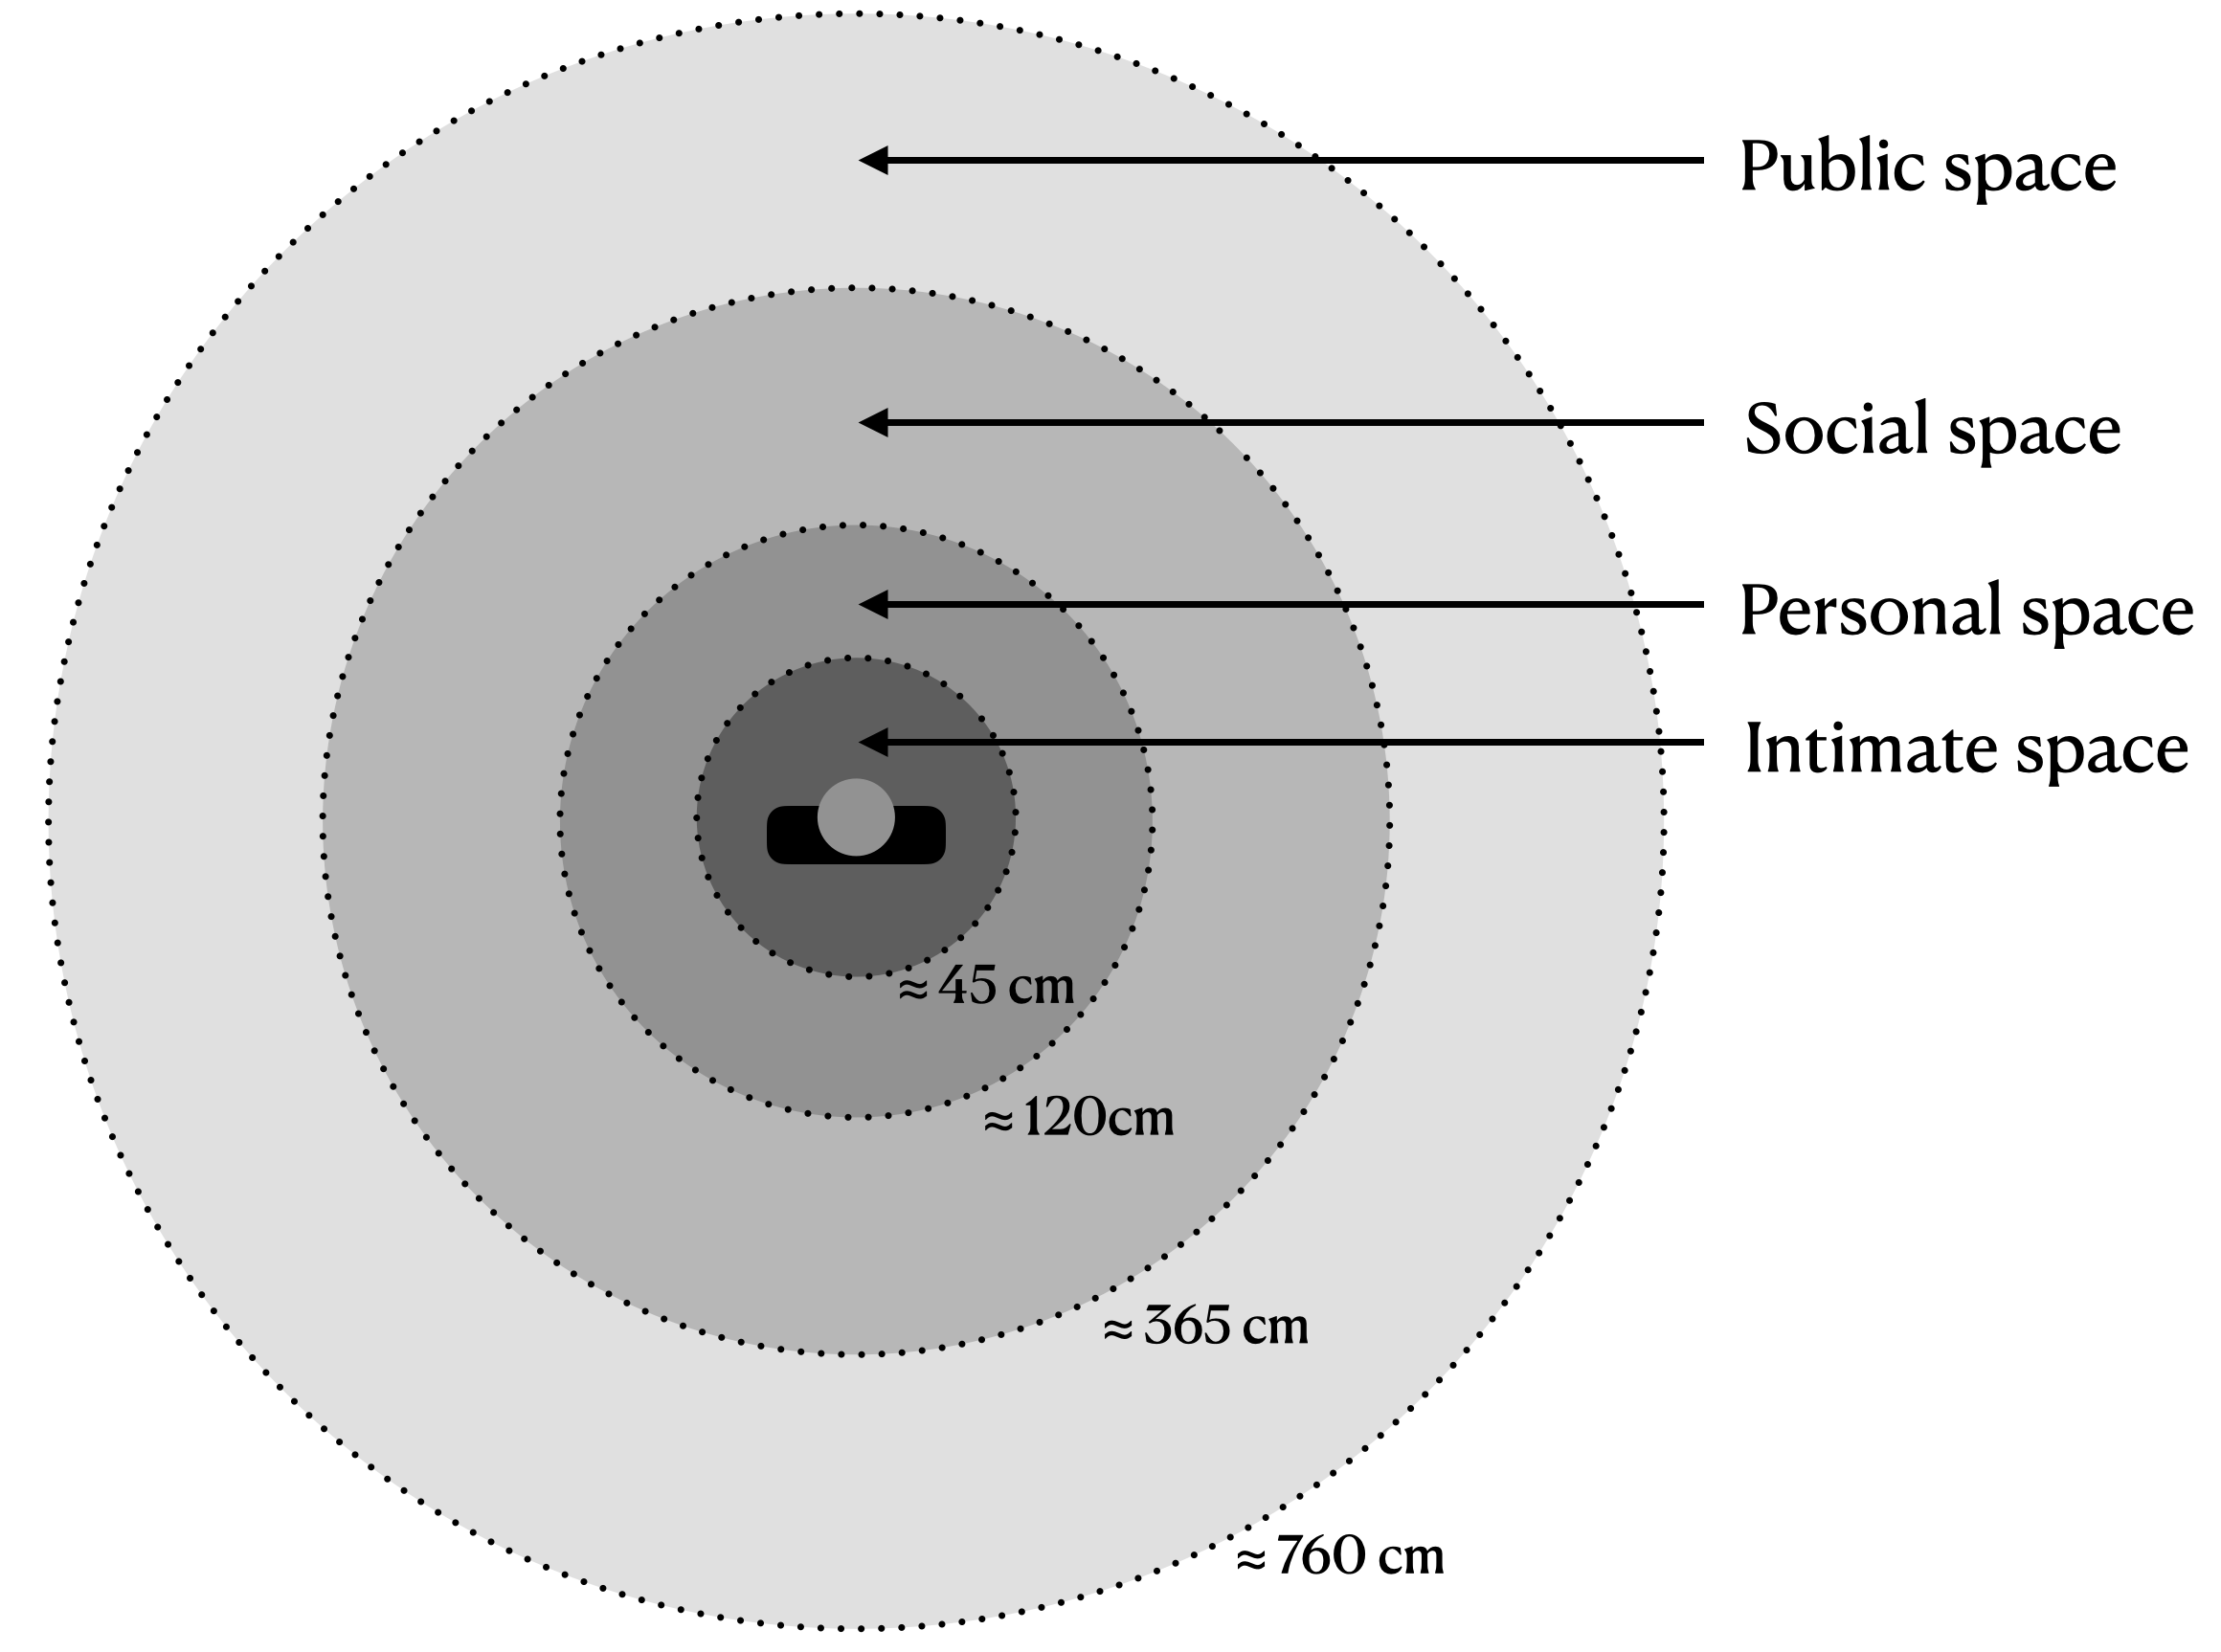
\includegraphics[width=9.5cm]{figs/personal_space.png}
\caption{Hall's model of the different spaces surrounding people.}
\label{personal}
\end{figure}

The innermost space, coined \textit{intimate space} are reserved for our closest relations which we embrace and physically touch. The next space, known as \textit{personal space}, is where we interact with friends and wider family. Following this is the \textit{social space} where acquaintances etc. are let in. Finally we have the \textit{public space} where strangers and impersonal interactions often occur. Note that in Europe the provided numbers might be substantially different, reports indicated that expected social distance there is roughly half what it is in the US \cite{hall1969hidden}. This is also varying between cultures and as mentioned in the introduction, situations like the COVID-19 pandemic can alter the established interpretation of social appropriate inter-personal distance.


Group behaviour has also been an important feature in the  social contexts simulated in this work. Kendon \cite{kendon1990conducting} introduced the term \textit{Free-standing conversational groups} (FCGs) \nomenclature{FCGs}{Free-standing conversational groups} and uses the concept of F-formation to describe the social-spatial formation that occur when people stand in groups. In this work we only simulate the classical circle-formation for groups but there exist multiple others such as ellipse, vis-a-vis, side-by-side or L-shape \cite{setti2015f}. Instead of group formation we investigate the impact of more group dynamics related terms such as inclusion and exclusion \cite{forsyth2018group}, as well as distance to groups and the mere presence of groups in a context. With respect to F-formations, we might not use this explicitly for groups of people, but they are still interesting when looking at axial orientation of people and robot during interactions, i.e. how they face each other. In Figure \ref{formation}, the different F-formations relevant for this work is presented, divided into how they are relevant for groups of people and how they might occur in human-robot situations.


\begin{figure}[h]
\centering
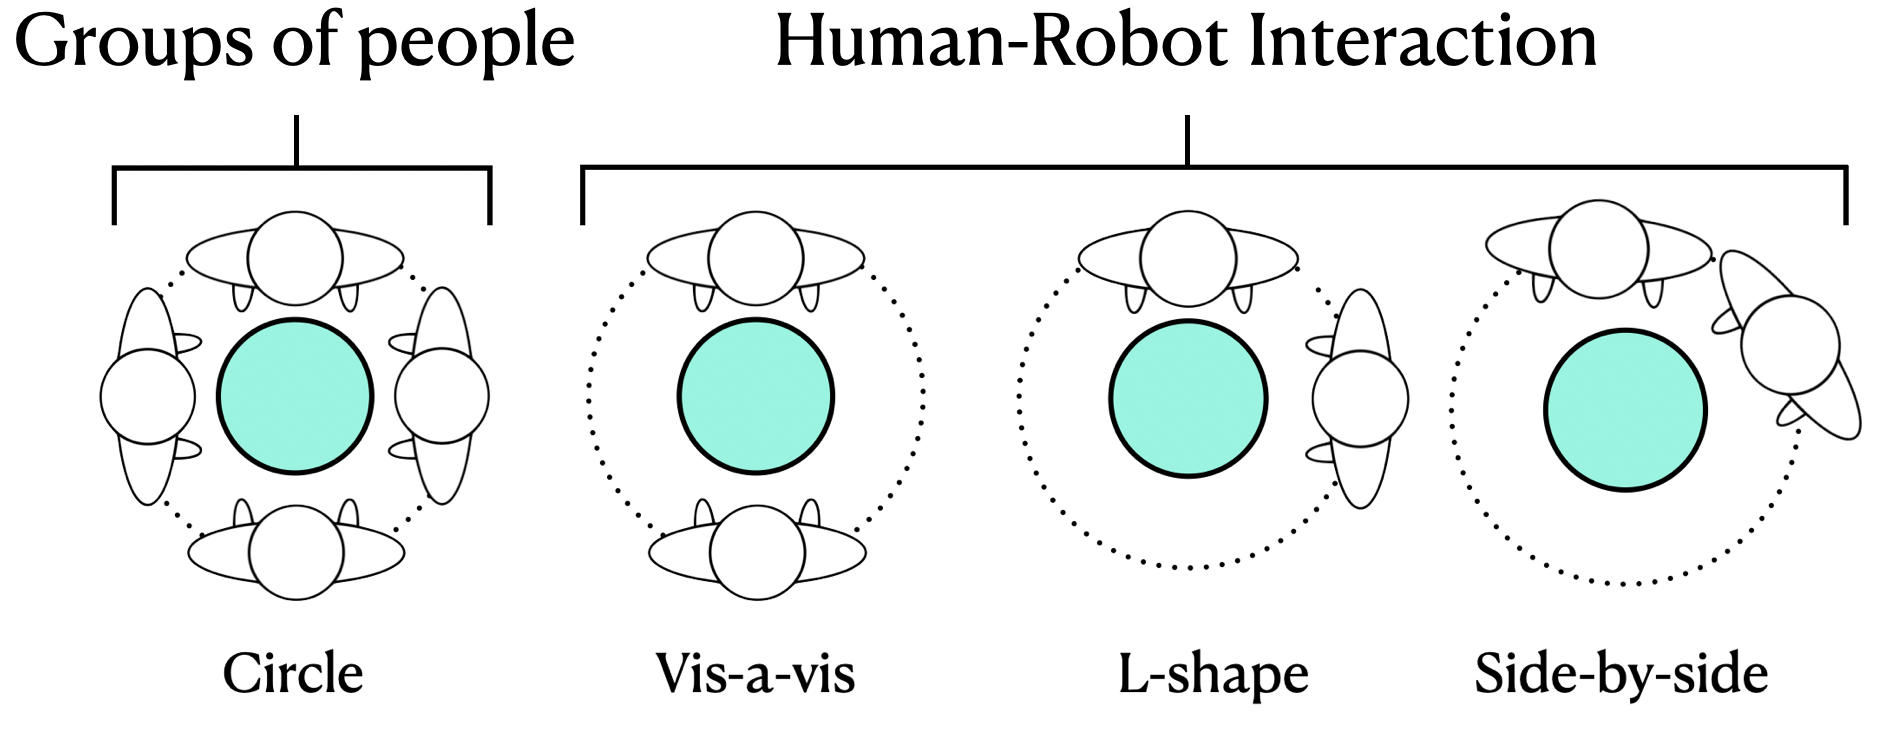
\includegraphics[width=13cm]{figs/formation.png}
\caption{The F-formations relevant to this work for groups of people (left) and human-robot interaction (right).}
\label{formation}
\end{figure}



\section{Social robotics}
Building on the foundation from the previous section on social contexts we will now include the robotics perspective. The field of social robotics is wide but this section will focus on interpersonal distance between human and robot as well as robot behaviour around and towards groups of people. 

Previous work show that robots are treated differently than humans with respect to appropriate interpersonal distance and invasion of personal space. Evidence show that when introduced to a robot, people prefer it to be positioned in the \textit{social space} and first during interaction do they feel comfortable allowing it into the \textit{personal space} \cite{huttenrauch2006investigating, walters2009empirical}. Studies show that these preferences change as people get used to the robot over time \cite{koay2007living}, and is dependent on robot appearance \cite{walters2008avoiding}. Most of the existing work on robot behaviour toward and around people have focused on socially aware motion planning \cite{triebel2016spencer} or approach \cite{walters2007robotic}, there are however some interesting research gaps which will be investigated further in the related work section. Researchers have also examined how and when to engage humans appropriately in HRI situations, based on sensory inputs indicating location, pose, and movement of humans in the environment \cite{michalowski2006spatial}.


\section{Deep learning}
Deep learning models have in recent years shown impressive behaviour in tasks ranging from complex board games \cite{go} to medical image classification \cite{derma}. Their ease of use and ability to learn high dimensional representations have reshaped how many of today's machine learning problems are approached.
This section briefly describes the foundations of deep learning before going into more detail about the sub-field of Bayesian deep learning, which is utilised in this work.

\subsection{Multilayer perceptron}
Multilayer perceptrons (MLPs), \nomenclature{MLP}{Multilayer perceptron} also called feedforward networks, aim to represent a function $f$ which can be viewed as a mapping from an input vector $\bm{x}$ to an output $ \bm{y} = f^{\bm{\omega}}(\bm{x})$ \cite{Goodfellow-et-al-2016}. Where $\bm{\omega}$ are the parameters which are learned through the steps of back-propagation \cite{rumelhart1986learning}. The networks consist of an input layer, varying numbers of hidden layers and an output layer. In each neuron of each layer, except the input layer, the weighted sum of the inputs and a bias term is computed and passed through an activation function, $\bm{\sigma}$, leading to the output. An illustration of a traditional MLP (inspired by figures in \cite{haykin1994neural}) as well as the details of the per-unit operations are presented below in Figure \ref{mlp}.

\begin{figure}[h]
\centering
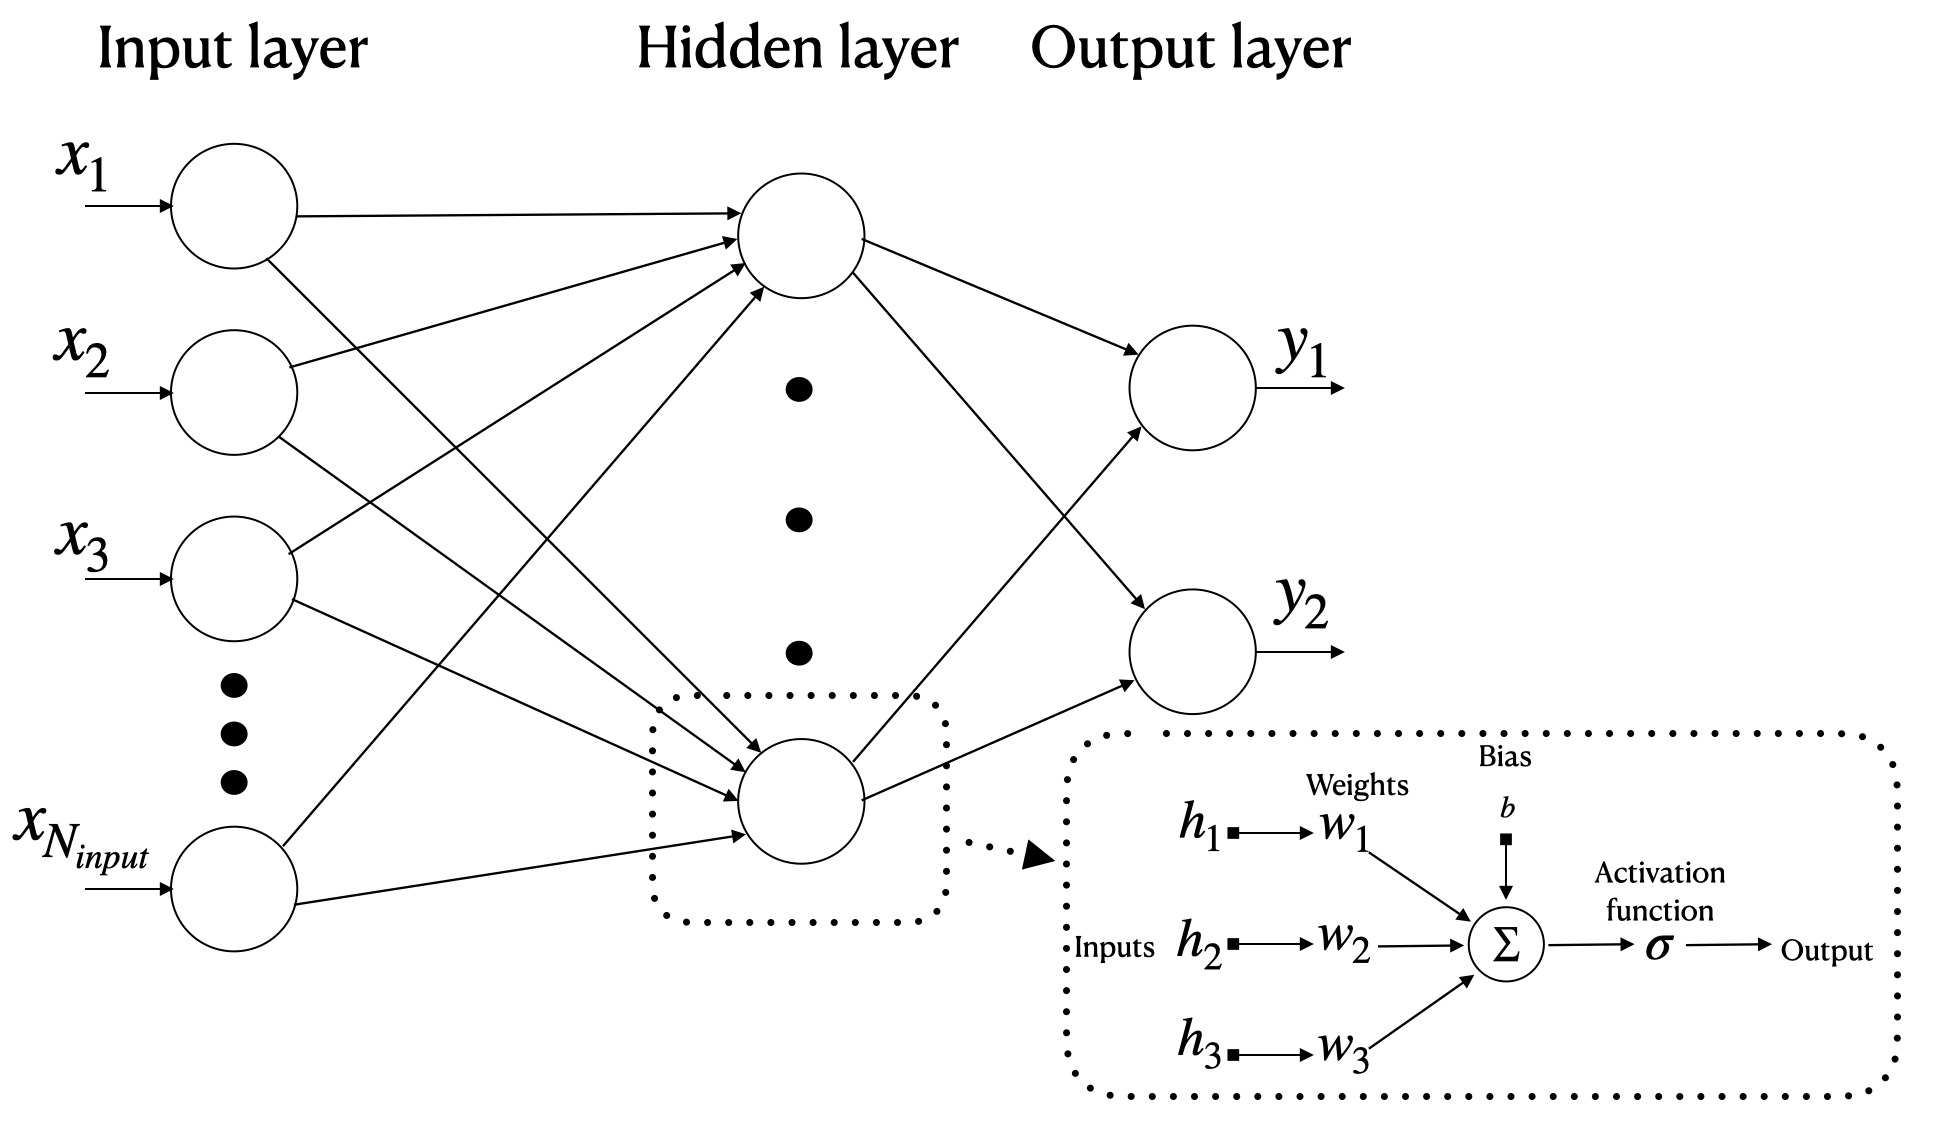
\includegraphics[width=13cm]{figs/mlp.png}
\caption{A traditional multilayer perceptron and the computation within a single unit of the network.}
\label{mlp}
\end{figure}

\subsection{Bayesian neural networks}
The idea of Bayesian neural networks (BNN) \nomenclature{BNN}{Bayesian neural network} is not new, but was in fact introduces by Neal \cite{neal2012bayesian} and McKay \cite{mackay1992practical} in the 90s. BNNs acts as function approximator equivalent to the MLP described above, but instead of point values for the neural network weights, BNNs place a prior distribution over the weights which further leads to a distribution over a parametric set of functions. In other words, they offer a probabilistic representation of classical deep learning models. Figure \ref{bnn} indicates the difference between a BNN and the traditional MLP, the weights are here represented by distributions instead of point values.

\begin{figure}[h]
\centering
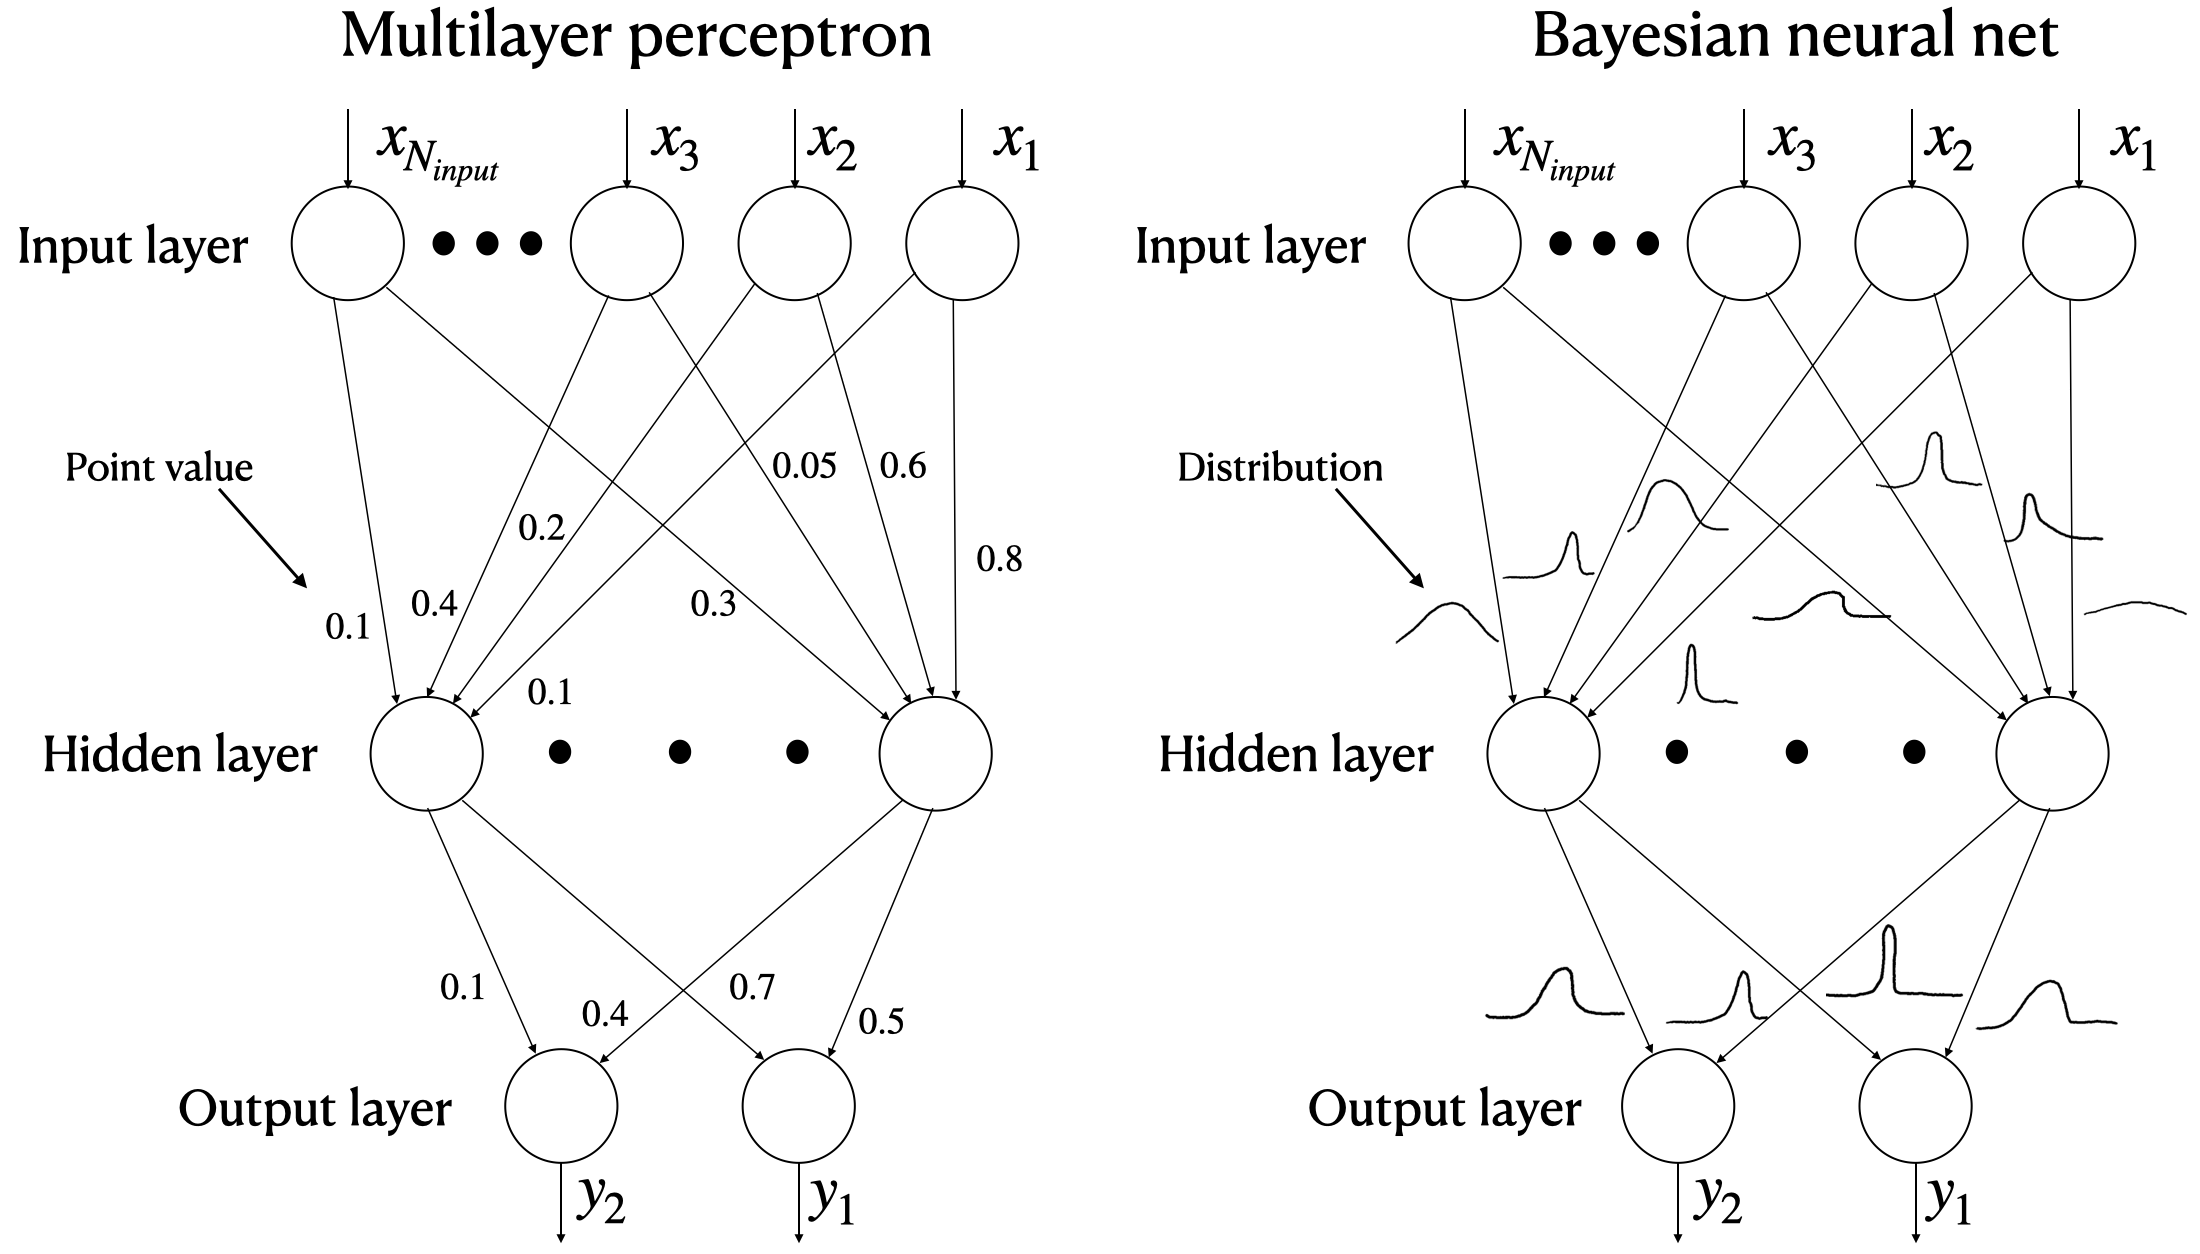
\includegraphics[width=13cm]{figs/bnn.png}
\caption{The distinction between a traditional Multilayer perceptron and a Bayesian neural net.}
\label{bnn}
\end{figure}

This inherent attribute of BNNs means that weight values can be sampled during inference, ultimately leading to a stochastic output which rich uncertainty estimates can be extracted from. Building on the description of the network models described in Section 2.2.1, we define the model likelihood of a BNN as $p(\bm{y}|f^{\bm{\omega}}(\bm{x}))$. The goal when training the network if given data, $\bm{X} = \{\bm{x_1}, \bm{x_2},..,\bm{x_N}\}, \bm{Y} = \{\bm{y_1}, \bm{y_2},..,\bm{x_N}\}$, is to find the posterior distribution over the weights, $p(\bm{\omega}|\bm{X},\bm{Y})$. This approach introduces multiple benefits such as robustness against over-fitting and a data-efficient training process when given a reasonable prior. However, BNNs leads to challenges at inference due to the intractability of the marginal probability, $p(\bm{Y}|\bm{X})$, which is needed to compute the posterior as seen below in Bayes theorem,

\begin{equation}
\label{bayes}
p(\bm{\omega}|\bm{X},\bm{Y}) = \frac{p(\bm{Y}|\bm{X},\bm{\omega})p(\bm{\omega})}{p(\bm{Y}|\bm{X})}.
\end{equation}

To handle this, several approximate inference techniques have been proposed over the years \cite{graves2011practical, hernandez2016black, hastings1970monte}, divided in two sub groups, variational inference (VI) \nomenclature{VI}{Variational inference} and sampling based methods. The Bayesian framework implemented in this work builds on the \textit{Bayes-by-backprop} (BBB) \nomenclature{BBB}{Bayes-by-backprop} method introduced by Blundell et al. \cite{blundell2015weight}, a back-propagation-compatible algorithm using the VI technique described in detail below.

As a variational inference technique, BBB transforms the inference problem into an optimization problem by defining a approximate variational distribution, $q_{\bm{\theta}}(\bm{\omega})$, and minimizing the Kullback-Leibler (KL) \cite{kullback1951information} \nomenclature{KL}{Kullback-Leibler} divergence between this and the true Bayesian posterior on weights, $p(\bm{\omega}|\bm{X},\bm{Y})$. Formally we try to find the parameters $\theta$, such that

\begin{equation} \label{KL}
\begin{split}
\theta^* & = \argmin_{\bm{\theta}} KL[q_{\bm{\theta}}(\bm{\omega})||p(\bm{\omega}|\bm{X},\bm{Y})]
\\
 & = \argmin_{\bm{\theta}} \int q_{\bm{\theta}}(\bm{\omega}) log \frac{q_{\bm{\theta}}(\bm{\omega})}{p(\bm{\omega}|\bm{X},\bm{Y})} \\
 & = \argmin_{\bm{\theta}} KL[q_{\bm{\theta}}(\bm{\omega})||p(\bm{\omega})]- \mathbb{E}_{q_{\bm{\theta}}(\bm{\omega})}[\log p(\bm{X},\bm{Y}|\bm{\omega})].
\end{split}
\end{equation}

 The resulting cost function from equation \eqref{KL} is known as \textit{variational free energy} or \textit{expected lower bound} (ELBO), \nomenclature{ELBO}{Expected lower bound} coined by Neal and Hinton among others \cite{neal1998view, saul1996mean}. To approximate this, Blundell et al. \cite{blundell2015weight} proposed a generalisation of the well-used Gaussian re-parameterisation trick \cite{kingma2013auto, opper2009variational, rezende2014stochastic}, operating on stochastic weights instead of stochastic hidden units like previous work. By leveraging this, the exact cost can be approximated as, 
 
\begin{equation}
\label{loss_BBB}
\Lagr_{BBB}(\bm{\theta},\bm{X},\bm{Y}) \approx \sum_{i = 1}^{M} 
\log q_{\bm{\theta}}(\bm{\omega_i}) - \log p(\bm{\omega_i}) - \log p(\bm{X},\bm{Y}|\bm{\omega_i}),
\end{equation}

where $\bm{\omega_i}$ represents the $i$th Monte Carlo sample from the variational posterior, $q_{\bm{\theta}}(\bm{\omega})$. Following the recommendations of Blundell et al. \cite{blundell2015weight} we implement a Gaussian variational posterior with mean, $\mu$, and standard deviation, $\sigma$, represented as $\bm{\theta} = (\mu, \sigma)$. The standard deviation is parametrised pointwise as $\sigma = \log(1+\exp{(\rho)})$, thus always non-negative. A posterior sample of the weights, $\bm{\omega}$, is sampled using the re-parameterisation trick, $\bm{\omega} = \mu + \sigma \circ \epsilon$, where $\epsilon$ represents noise sampled from a unit Gaussian which are pointwise multiplied with $\sigma$. The second term in equation \eqref{loss_BBB} represents the prior over the weights. As suggested in previous work \cite{blundell2015weight}, this is implemented as a scale mixture of two Gaussian densities, both zero centered but with different variances, $\sigma_1, \sigma_2$. The last term of equation \eqref{loss_BBB} denotes the model likelihood which will be explained more in detail and specifically for our framework in Chapter 5.

\section{Predictive uncertainty in deep learning}
When covering this topic there is no way around referencing Yarin Gal's PhD thesis on \textit{Uncertainty in Deep Learning} \cite{gal2016uncertainty}. His thesis gives a great review of the field, as well as several substantial contributions used widely today. We will build on some of his thoughts when defining predictive uncertainty in deep learning below. A fundamental part of this project rests on the separation between Aleatoric and Epistemic uncertainty, also called irreducible and reducible uncertainty. Together, they make up rich, predictive uncertainty estimates for machine learning. 

Aleatoric uncertainty captures the inherent noise in the data, in other words, uncertainty that cannot be explained by adding more observations. A typically example is a dice roll, no number of observed rolls will completely remove the uncertainty in the outcome of the next one, it is inherently stochastic. Note however that using the term irreducible might be misconceiving, in some cases noisy data can come from faulty  sensor measurements, which in fact can be reduced. Further, we can separate between heteroscedastic and homoscedastic Aleatoric uncertainty. The homoscedastic approach, first introduced in the neural network setting by Nix and Weigend \cite{nix1994estimating}, assumes that the observation noise is constant over the input space, i.e. identical for every input. Heteroscedastic uncertainty on the other hand, allows the aleatoric uncertainty to vary with the input, predicting higher uncertainty in parts of the observation space where the inherent noise is bigger \cite{le2005heteroscedastic}. In our work, heteroscedastic aleatoric uncertainty is used because we are interested in distinguishing between  input data that leads to high agreement among people versus scenes people tend to disagree about. 

Epistemic uncertainty, also called model uncertainty, can show up in two ways. We either talk about \textit{out out distribution} data, for example when an image classifier trained on pictures of dogs is shown a picture of a cat and expected to give a prediction. Ideally, if incorporating epistemic uncertainty, the model should indicate that it has never seen data like this before and is therefore not able to make a reasonable decision. Similarly, but slightly different, would be models with access to only sparse data on certain parts of the observation space which then should lead to higher epistemic uncertainty then for samples that frequent often. This would not be an \textit{out out distribution} scenario, but rather a \textit{lack of data} situation, for example the  same dog classifier given a picture of a white dog, but most of the training data contains dogs with dark coats.

Kiureghian and Ditlevsen argued the importance of using these separate uncertainty estimates in engineering modeling \cite{der2009aleatory} and Kendall and Gal first introduced a practical way of combining the two into a single model \cite{kendall2017uncertainties}. Their method is the one implemented in this work, more detail will be provided in the related work chapter.

\section{Continual Learning}
As mentioned in the introduction, humans have the ability to continuously acquire and develop their knowledge about the world and surrounding environment. Not only do we update what we currently know when new information arrives, but sensorimotor skills and long-time memory abilities ensures that we do not forget previous experiences. This term is often coined Lifelong \cite{thrun1995lifelong, chen2016lifelong} or Continual learning (CL) \nomenclature{CL}{Continual learning}  \cite{ring1994continual} and has for long been a difficult challenge for the machine learning and neural network community. Following the definitions of Lesort et al. \cite{lesort2020continual} we will use the term Continual learning throughout this work which might overlap with other established terms such as Incremental learning \cite{gepperth2016incremental} and Never-ending learning \cite{carlson2010toward}. In essence, Continual learning covers the approaches that handle the challenge of learning new tasks sequentially with a continuous stream of data, where the data distribution might change over time and where old data not always is available. In this section we will present some of the definitions and challenges within CL that are relevant to our implementation.

In the case of deep learning, the phenomenon of catastrophic forgetting \cite{french1999catastrophic} or catastrophic inference \cite{mccloskey1989catastrophic}, is often mentioned as the biggest challenge in Continual learning. This occurs when a neural network is trained sequentially on new concepts, for example first shown images of cats, with the goal of labelling them, followed by the same approach for images with dogs. What might happen is that the network overrides its knowledge about cats to optimize its ability to classify dogs. In this project we implement a CL method from previous work that mitigates catastrophic forgetting using uncertainty \cite{ebrahimi2019uncertainty}. 

Following this, we define some important terms necessary to understand the Continual learning approach in our work. We differ between learning new tasks vs learning actions or classes. A classical example could be an image classifier which in a CL setting learned to classify the numbers from 0-9 in two tasks. The first task could be to learn to recognize the numbers from 0-4, i.e. 5 classes but one task, followed by the second task of learning the numbers from 5-9. In other words, a Continual learning model learns new tasks sequentially, but every task can consist of multiple classes, or actions in a robotics scenario. In our case the robot learns the social appropriateness of multiple actions which can be acquired sequentially over several tasks. It is also important to emphasise the type of change in data when moving between tasks. This can be framed into three categories \cite{lesort2020continual}:
\newpage
\begin{itemize}
  \item \textbf{New Concepts:} At task $t$ the data distribution of the input is the same as for previous tasks, but the predicted variable $Y$ (actions/classes), is a new dependent variable to be learned.
  \item \textbf{New Instances:} At task $t$ the data distribution of the input might be different then for previous tasks, but the predicted variable $Y$ (actions/classes), is the same as the one used in the past
  \item \textbf{New Instances and New Concepts:} A combination of the two above, both the data distribution of the input as well as the variable to predict change over tasks.
\end{itemize}

The above-mentioned image classifier is an example of both new instances and new concepts. Input data, the image, look different from task to task and the variables to predict, classes 0-4 and 5-9, respectively, also change. For the social robotic application in this work, the model is only give access to new concepts not instances, this will be explained more in Chapter 5.

Another important aspect of continual learning strategies is how the CL model's architecture is modified or kept constant throughout learning. Some well-used strategies are: \textit{Explicit architecture modification}, where a new model is created for each new task and then connected to all previous models \cite{rusu2016progressive}, \textit{Implicit architecture modification}, where the architecture itself is not modified, but some weights are freezed to mitigate catastrophic forgetting \cite{mallya2018packnet}, and \textit{Dual architectures}, where one model is used as memory and one for learning new tasks, often seen in bio-inspired approaches \cite{furlanello2016active}. In our work we implement a hybrid of an explicit and implicit architecture modification, where the update rate of some weights are limited to remember previous experiences, but the final layer is also modified based on number of tasks to learn.


\chapter{Related Work} 
\section{Social appropriateness in robotics}
As mentioned in the background chapter, most work on this topic has revolved around socially aware motion planning. In addition, the recent rise in popularity for deep learning models have yet to make a substantial breakthrough in social appropriate robotics where previous work have focused more on the use of handcrafted and extensively feature engineered methods. However, some researchers have leveraged modern machine learning techniques for the problem of social appropriateness in robotics. Chen et al. used Deep reinforcement learning (DRL) \nomenclature{DRL}{Deep reinforcement learning} to teach a wheeled robot socially compliant navigation \cite{chen2017socially}. They approached the challenge of socially appropriate motion planning by emphasizing what the robot \textit{should not do} instead of what it \textit{should do}. Also using DRL, Gao et al. \cite{gao2019learning} investigated how robots should approach groups of people in a socially appropriate way on the same humanoid robot, Pepper \cite{pepper}, used in our work. Similarly, human-aware navigation have been proposes through the use of "social forces" interacting between humans and robot companions \cite{ferrer2013robot}. While all of these are interesting approaches to the challenge of motion planning in a human environment, neither of them investigate the social appropriateness of a wider range of robot actions.

In the introduction we briefly introduced how determining the social appropriateness of an action can begin by determining the social context of which that action will be executed. Contextual understanding have for long been important in Human computer interaction (HCI) \nomenclature{HCI}{Human computer interaction} \cite{dey2001understanding}, and several works in the field of HRI have aimed to model context \cite{mastrogiovanni2009context, larochelle2011establishing}. Çelikkanat et al. neatly transferred the classical topic modeling method, Latent Dirichlet Allocation (LDA), \nomenclature{LDA}{Latent Dirichlet Allocation} and used it to model contexts instead \cite{celikkanat2015learning}. It is worth noting that they also implemented an incremental model comparable to the one used in this project. All of the above-mentioned works try to model contexts only, which thereafter can be used to determine suitable robot actions. We, however, implement an end-to-end solution, mapping directly from the feature space obtainable through sensory inputs to the social appropriateness of actions. Slightly closer to our work is Rosenthal et al. \cite{rosenthal2020context}, which investigate the social appropriateness of a robot delivering a message in three different contexts. However, while this is similar to how we approach the challenge of learning appropriate actions, Rosenthal et al. only presents insight from surveys, they do not develop any machine learning models.

\section{Rich uncertainty estimates}
As mentioned in the background, Kendall and Gal were the first to introduce a model able to combine aleatoric and epistemic uncertainty \cite{kendall2017uncertainties}. They leveraged the practical dropout approach \cite{gal2016dropout} for variational Bayesian approximation to capture epistemic uncertainty. By implementing dropout before every fully-connected layer in the network, both during training and test time, stochastic forward passes are sampled. This is referred to as Monte Carlo dropout and has been proven formally to be equivalent to the approximate variational inference method described in the background chapter, where the Kullback-Leibler divergence is minimised. In our work we achieve the same by running multiple stochastic forward passes through the Bayesian neural network. Further, Kendall and Gal includes heteroscedastic aleatoric uncertainty by extending the model output to predict  both a mean, $\hat{y}$, and a variance, $\hat{\sigma}^2$. Other recent works have proposed more straightforward ways of doing the same, mostly in image classification and segmentation applications \cite{kwon2018uncertainty, shridhar2018uncertainty}. Our work is different in that we implement the method in a continual learning application and use a BNN instead of Monte Carlo dropout to facilitate for it. In addition, all of the above-mentioned work using rich uncertainty estimates have been applied to computer vision challenges. A social robotics implementation taking use of both aleatoric and epistemic uncertainty is, to our knowledge, novel.

\section{Uncertainty guided continual learning}
This project implements the uncertainty guided continual learning strategy, (UCB), \nomenclature{UCB}{Uncertainty guided continual learning} proposed by Ebrahimi et al. \cite{ebrahimi2019uncertainty}. They handled the challenge of catastrophic forgetting by slowing down learning on weights important for previous task, similar to Kirkpatrick et al. \cite{kirkpatrick2017overcoming}. However, they identified parameter-importance in a novel way, by using the weight uncertainty inherent in BNNs. The key benefits of their algorithm is that you do not need to add additional memory, track parameter change throughout learning or explicitly be aware of when a new task arrive, with respect tot the learning rate updates. This section will briefly cover their proposed strategy.

As described in the background chapter, in a Bayesian neural network every weight is a distribution represented by a mean and a variance, different from the traditional MLP which uses point values for every weight. Ebrahimi et al. leverages this and defines the importance of a network parameter according to the current variance of that parameter. To facilitate for continual learning, without forgetting previous knowledge, they update the per-parameter learning rate as the overall learning rate for the model times the parameter variance. It is worth noting that Ebrahimi et al. found empirically that only the learning rate for the  parameters' mean, $\mu$ should be adapted like this and that not adapting the learning rate for, $\rho$, in the parametrised standard deviation, yields the best results. Algorithm \ref{algo} presents the straightforward update rules for each parameter in the UCB strategy for mitigating catastrophic forgetting, taken directly from the initial paper.

\begin{algorithm}
\caption{Learning rate update in UCB }\label{algo}
\begin{algorithmic}[1]
\State \textbf{function} LearningRateUpdate($\alpha_{\mu}, \alpha_{\rho}, \sigma$)
\For{each parameter}
    \State $\Omega_{\mu} \leftarrow 1/\sigma$
    \State $\Omega_{\rho} \leftarrow 1$
    \State $\alpha_{\mu} \leftarrow \alpha_{\mu}/\Omega_{\mu}$
    \State $\alpha_{\rho} \leftarrow \alpha_{\rho}/\Omega_{\rho}$
\EndFor
\end{algorithmic}
\end{algorithm}

Here, $\Omega_{\mu}$ and $\Omega_{\rho}$ represents the per-parameter importance factor for the mean and parametrised variance, respectively. Following this, the per-parameter learning rates, $\alpha_{\mu}$ and $\alpha_{\rho}$ is updated by division with the importance factor, ultimately decreasing the learning rate on weights important for previous tasks. Figure \ref{ucb} illustrates this and show how the learning rate adapts with respect to the uncertainty in the weights throughout the continual learning process.

\begin{figure}[h]
\centering
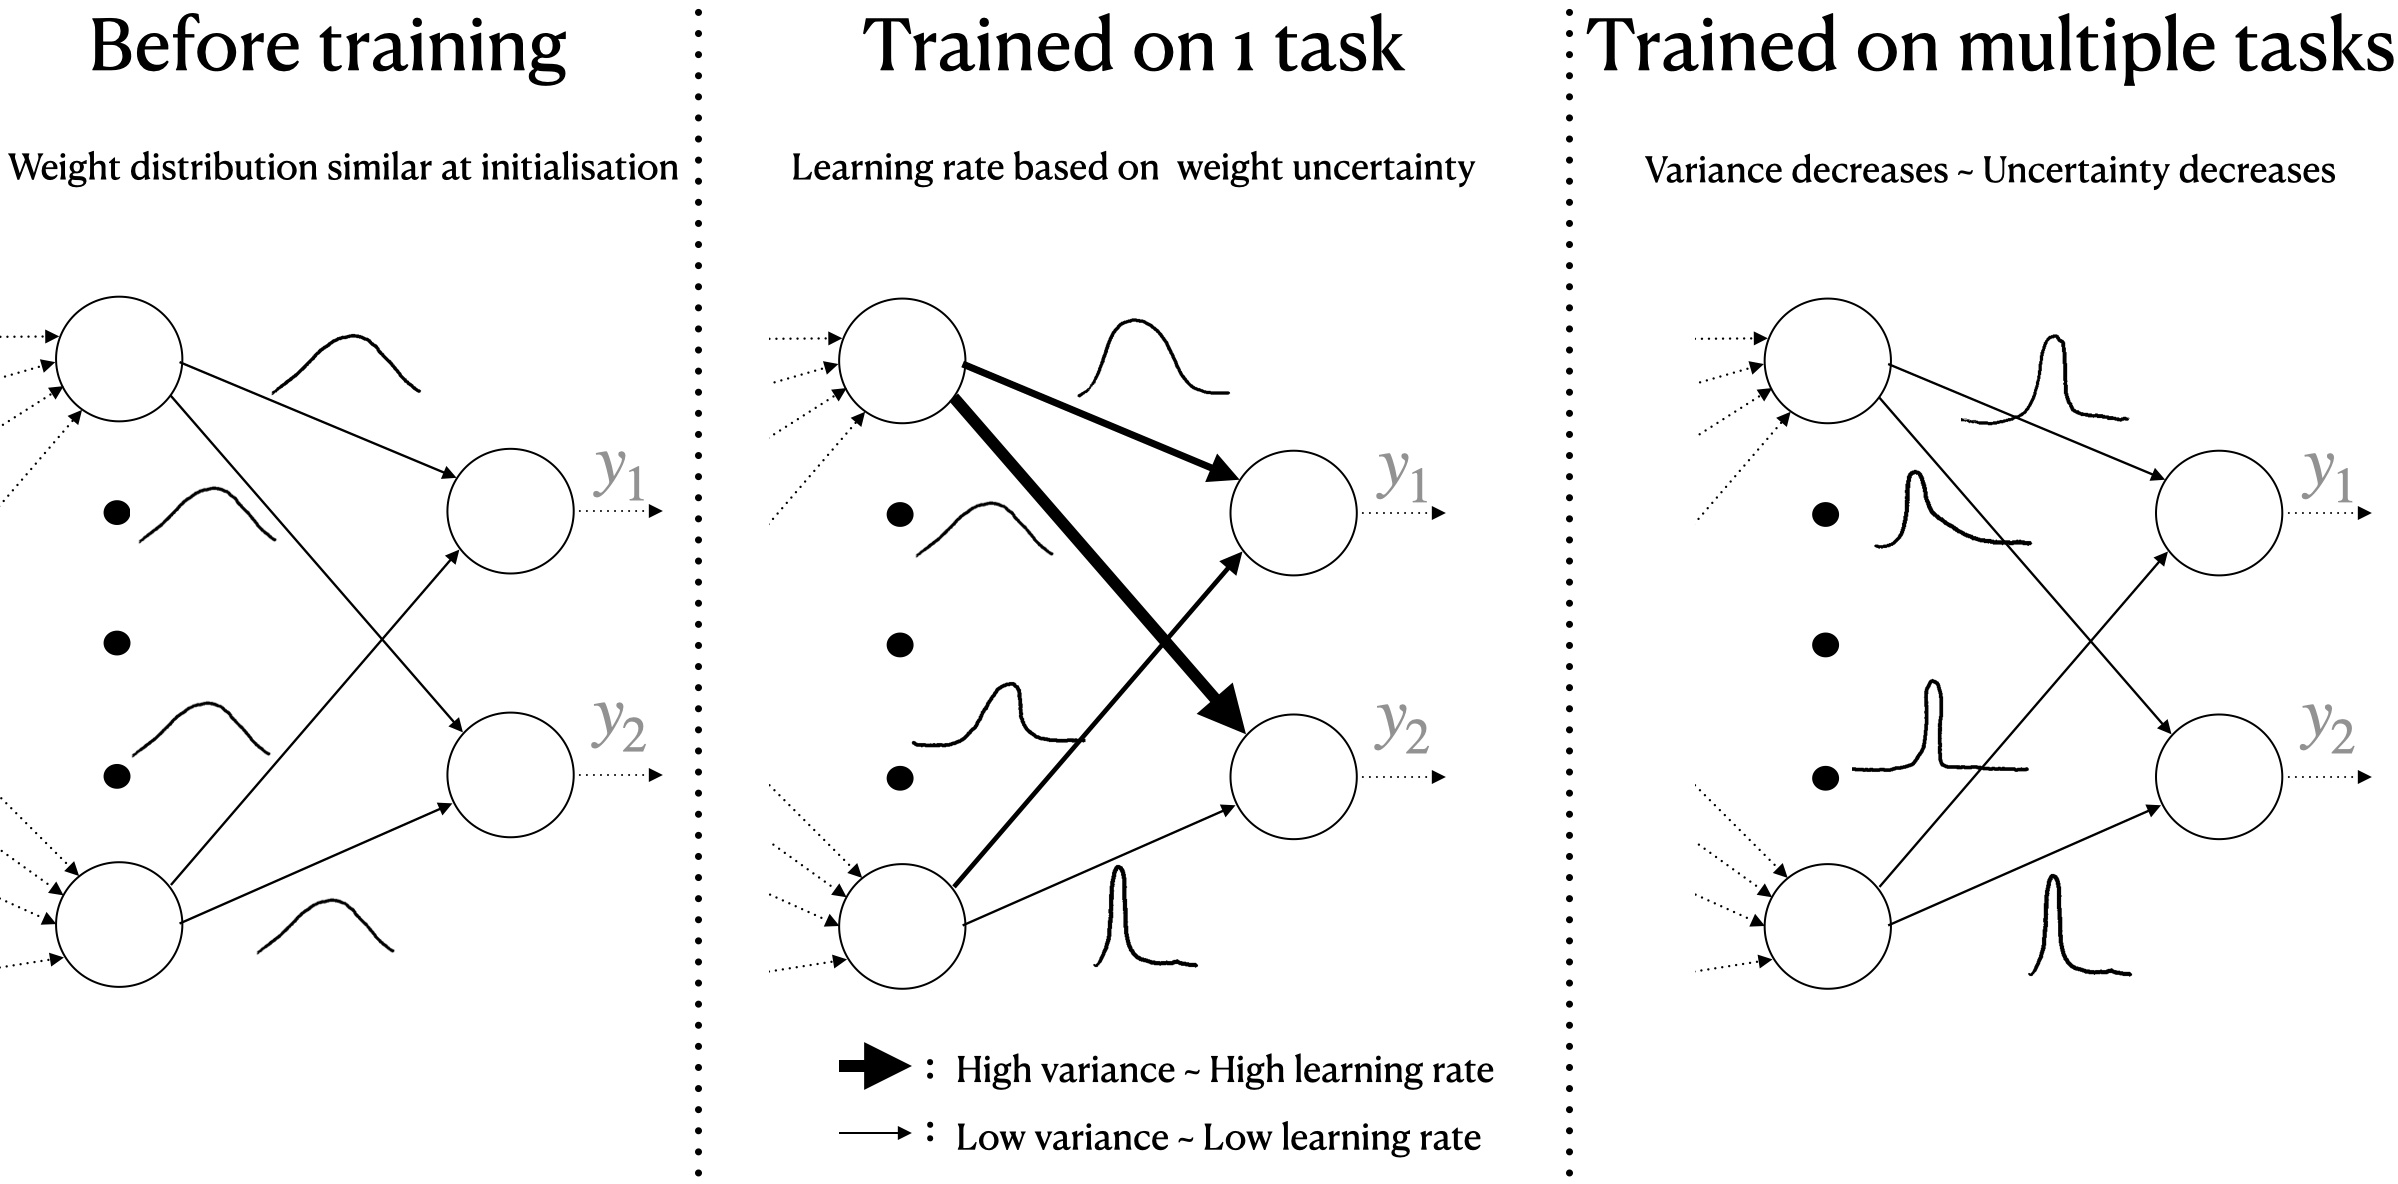
\includegraphics[width=13.5cm]{figs/ucb.png}
\caption{Showing how less certain weights are updated at a higher rate than more certain weights.}
\label{ucb}
\end{figure}

\chapter{Data}
A key contribution of this work is the the dataset of robot actions in a social living-room context, created from scratch, and labeled through a crowd-sourcing platform. In this chapter we will first go into detail about the simulation environment, before a thorough review of the feature engineering is given. Following this we provide some insight in the crowd-sourcing process. Finally, we present an analysis of the data, covering the social signals introduced in the background chapter as well as an investigation into annotator agreement.

\section{Simulation environment}
To simulate the different social contexts used to determine the appropriateness of certain robot actions, we use the Unity3D simulation software \cite{unity}. The living room in which all the scenes are generated is part of an Unity Asset package from Craft Studios \cite{apartment}. All avatars used to represent either people or animals are taken from Adobe's Mixamo software \cite{avatar}. Avatars are spawned into the living room scene as Unity Gameobjects, following a script in the Unity compatible C\# programming language.


\section{Feature engineering}
\section{Crowd-sourcing data}
- Crowd labeling, Prolific, Qualitrics, Figure 8

\section{Data analysis}
- Data analysis, personal space, agreement, etc.

\chapter{Bayesian Continual learning framework}
\section{Bayesian neural network models}
- Architecture
\\
- 3 Types, baseline, 2 tasks, 16 tasks
\\
\section{Continual learning approach}
- Parameter search
\\
\section{Extracting uncertainty estimates}
- Aleatoric, looking at both per task/action and mean
\\
- Epistemic, looking at both per task/action and mean. Different for baseline with no CL. Sample only last layer when CL. Investigate CL impact on Epistemic uncertainty.


\chapter{Evaluation} 
\section{Predictive performance}
- Show some scenes from unseen data and corresponding predictions.
\\
- Table with quantitative performance for all 3 models.

\section{Uncertainty estimates}
- Overall and task specific.
- How does it change when continually learning.


\chapter{Summary and Conclusions} 

\appendix
\singlespacing

\bibliographystyle{unsrt} 
\bibliography{bib.bib} 

\end{document}